\StartChapter{Differentialrechnung}

\SubsectionBar{Ableitungsregeln\ZSFScriptRef{63,65}}

\textVorBox{Die \ZSFkeyword{Ableitung} beschreibt die Änderungsrate einer Funktion.}

\begin{fulltablebox}{Q{0.8} | Y{1.2}}
    \ZSFrowColor
    Potenz: & $\displaystyle (x^n)' = nx^{n-1}$ \\ \hline
    Addition: & $\displaystyle (f(x) + g(x))' = f'(x) + g'(x)$ \\ \hline
    \ZSFrowColor
    Multiplikation: & $\displaystyle (f(x)g(x))' = f'(x)g(x) + f(x)g'(x)$ \\ \hline
    Faktor: & $\displaystyle (cf(x))' = cf'(x)$ \\ \hline
    \ZSFrowColor
    Division: & $\displaystyle \left(\frac{f(x)}{g(x)}\right)' = \frac{f'(x)g(x) - f(x)g'(x)}{g^2(x)}$ \\ \hline
    Verkettung: & $\displaystyle (f(g(x)))' = f'(g(x))g'(x)$ \\ \hline
    \ZSFrowColor
    Inverse: & $\displaystyle \left(f^{-1}(x)\right)' = \frac{1}{f'\left(f^{-1}(x)\right)}$ \\
\end{fulltablebox}

Die Ableitung einer geraden Funktion ist ungerade und umgekehrt.

\textVorBox{Sei $f$ eine gerade Funktion, so gilt für die ungeraden Ableitungen:}
\begin{formulabox}
    $\displaystyle f'(0) = f'''(0) = f'''''(0) = \dots = 0$
\end{formulabox}

\textNachBox{\ZSFdanger{Achtung:} Bei der Ableitung einer Wurzel den Faktor der Potenz sowie die innere Ableitung nicht vergessen.}

\SubsectionBar{Linearisieren \& Fehlerrechnung\ZSFScriptRef{64}}

Die Linearisierung ist ein Verfahren, um eine nichtlineare Funktion an einer Stelle $x_0$ durch eine lineare Funktion zu approximieren.\\
\textVorBox{Die Formel der \ZSFkeyword{linearen Ersatzfunktion} lautet:}

\begin{formulabox}
    $\displaystyle t(x) = f(x_0) + f'(x_0)(x - x_0)$
\end{formulabox}

\textNachBox{wobei $f(x_0)$ der Stützpunkt, $f'(x_0)$ die Steigung und $(x - x_0)$ der horizontale Abstand zu $x_0$ ist.}

\textVorBox{Der \ZSFkeyword{absolute Fehler} durch die Linearisierung beträgt:}

\begin{formulabox}
    $\displaystyle \Delta f = f(x) - f(x_0) \approx f'(x_0)(x - x_0)$
\end{formulabox}

\SubsectionBar{Mittelwertsatz \& Satz von Rolle\ZSFScriptRef{64}}

Der \ZSFkeyword{Mittelwertsatz} besagt, dass es zwischen zwei Endpunkten einer Funktion mindestens einen Punkt gibt, in dem die Tangente an die Funktion parallel zur Geraden durch die Endpunkte verläuft.\par
Der \ZSFkeyword{Satz von Rolle} besagt, dass bei einer differenzierbaren, nicht injektiven Funktion $f: (a, b) \to \R$ ein Punkt existieren muss, dessen Ableitung 0 beträgt.

\SubsectionBar{Kurvendiskussion\ZSFScriptRef{65}}

\textVorBox{Die \ZSFkeyword{Kurvendiskussion} dient dazu, eine Vorstellung von der Form einer Funktion zu erhalten:}

\begin{fulltablebox}{Y{1} | Y{1}}
    \ZSFrowColor
    \textbf{Positiv} & \textbf{Negativ} \\
    $\displaystyle f(x) > 0 \; \forall x$ & $\displaystyle f(x) < 0 \; \forall x$ \\ \hline
    \ZSFrowColor
    \textbf{Monoton wachsend} & \textbf{Monoton fallend} \\
    $\displaystyle f'(x) \ge 0 \; \forall x$ & $\displaystyle f'(x) \le 0 \; \forall x$ \\ \hline
    \ZSFrowColor
    \textbf{Konvex} («Tal/Loch») & \textbf{konkav} («Berg») \\
    $\displaystyle f''(x_0) > 0$ & $\displaystyle f''(x_0) < 0$ \\
\end{fulltablebox}

\begin{fulltablebox}{Z{1} | Z{1} | Z{1}}
    \ZSFrowColor
    \textbf{Lokales Minimum} & \textbf{Lokales Maximum} & \textbf{Wendepunkt} \\
    $\displaystyle f'(x_0) = 0$ \par $f''(x_0) > 0$ & $\displaystyle f'(x_0) = 0$ \par $f''(x_0) < 0$ & $\displaystyle f'(x_0) = 0$ \par $f''(x_0) = 0$ \\
\end{fulltablebox}

\textNachBox{Wenn $f'(x) = f''(x) = \dots = f^{(n-1)}(x) = 0$ und $f^{(n)}(x) \neq 0$:\par
\dots ist $x$ eine lokale Extremalstelle, wenn $n$ gerade ist.\\
\dots ist $x$ ein Wendepunkt, wenn $n$ ungerade ist.}

\SubsectionBar{Tangenten}

Die \ZSFkeyword{Tangente} $t(x)$ an eine Funktion $f(x)$ in einem Punkt $x_0$ ist die Gerade, die an diesem Punkt dieselbe Steigung wie die Funktion besitzt. Es gilt $t(x_0) = f(x_0)$ und $t'(x_0) = f'(x_0)$.\par
Die Tangenten an $\cos(x)$ und $\sin(x)$ können nie eine Steigung besitzen, die im Betrag grösser ist als 1.

\SubsectionBar{Kurven\ZSFScriptRef{67}}

Im Gegensatz zu Funktionen können \ZSFkeyword{Kurven} jeden möglichen Verlauf annehmen. Sie können sich schneiden oder mehrmals denselben Wegabschnitt durchlaufen.\par
\textVorBox{Bei der \ZSFkeyword{Parameterdarstellung} werden die Punkte einer Kurve als Funktion eines oder mehrerer Parameter durchlaufen:}

\begin{formulabox}
    $\displaystyle t \to \vec{r}(t) = (x(t), y(t))$
\end{formulabox}

\textNachBox{Bei der \ZSFkeyword{impliziten Darstellung} $F(x,y) = 0$ wird die Funktion nicht nach einer der beiden Variablen aufgelöst.\par
Bei der \ZSFkeyword{expliziten Darstellung} $f(x)$ steht eine Variable allein auf einer Seite des Gleichheitszeichens.
\begin{itemize}
    \item[$\Rightarrow$] Bei der Umrechnung von der Parameter- in die explizite Darstellung nach $t$ auflösen und gleichsetzen.
\end{itemize}}

\textVorBox{Kurven können in \ZSFkeyword{polaren Koordinaten} ($\cos(\varphi) \cdot \rho(\varphi),\, \sin(\varphi) \cdot \rho(\varphi)$) dargestellt werden:}

\begin{formulabox}
    $\displaystyle x(\varphi) = \rho(\varphi)\cos(\varphi), \quad y(\varphi) = \rho(\varphi)\sin(\varphi)$
\end{formulabox}

\textVorBox{wobei $\rho(\varphi)$ die Distanz zum Koordinatenursprung ist:}

\begin{formulabox}
    $\displaystyle \rho(\varphi) = \sqrt{x(\varphi)^2 + y(\varphi)^2}, \quad \varphi = \arctan\left(\frac{y(\varphi)}{x(\varphi)}\right)$
\end{formulabox}

\columnbreak

\SubsectionBar{Ebene Kurven (S.67,68,69)}

\begin{defbox}[Kreis (Radius $R$, Mittelpunkt $(x_0, y_0)$)]
\begin{splitbox}[0.3]
    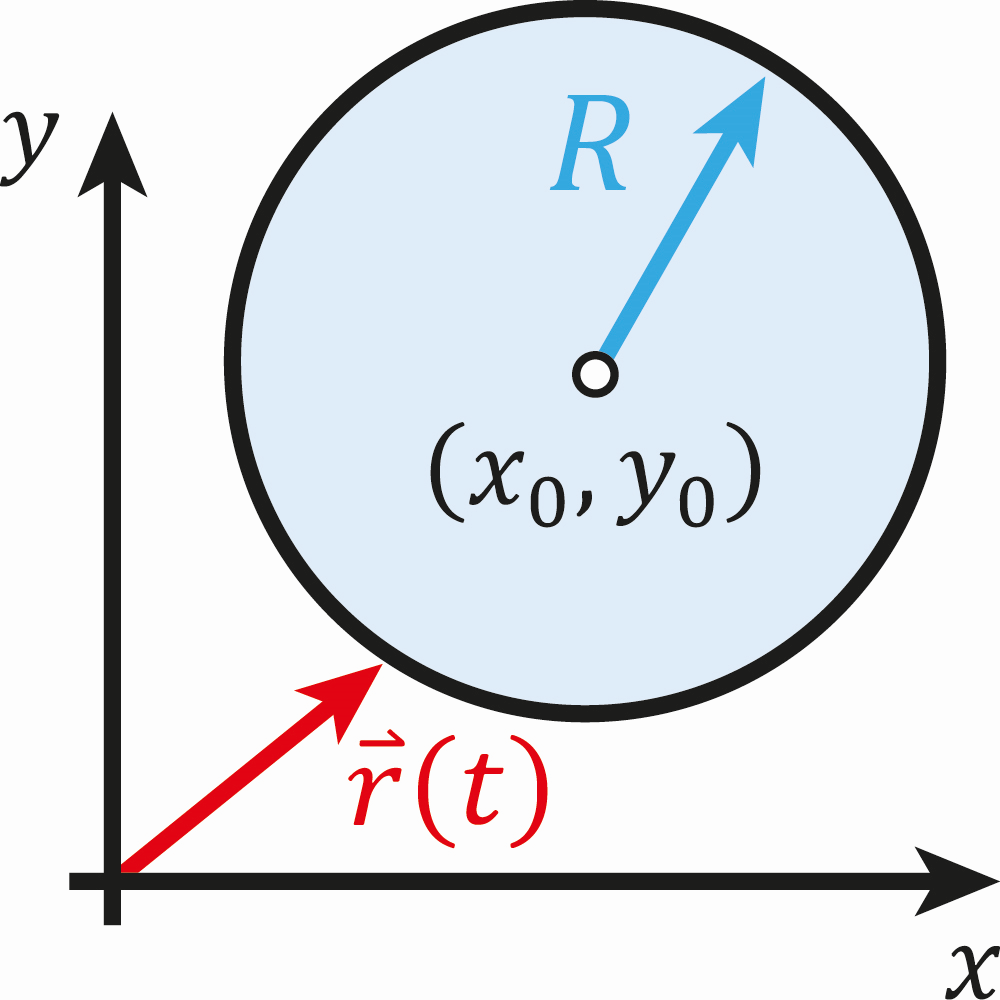
\includegraphics[width=\linewidth, keepaspectratio]{graphics/media/kreis_skizze.png}
    \tcblower
    \begin{formulabox}
        \textVorFormel{Parametrisiert mit $t \in [0,2\pi]$:}
        $\vec{r}(t) = (x_0 + R\cos(t), y_0 + R\sin(t))$\par
        \tcbline
        \textVorFormel{Implizit:}
        $(x - x_0)^2 + (y - y_0)^2 = R^2$\par
        \tcbline
        \textVorFormel{Explizit:}
        $f(x) = y_0 \pm \sqrt{R^2 - (x - x_0)^2}$
    \end{formulabox}
\end{splitbox}
\end{defbox}

\begin{defbox}[Ellipse (Mittelpunkt $(x_0, y_0)$ und Halbachsen $a, b$)]
\begin{splitbox}[0.3]
    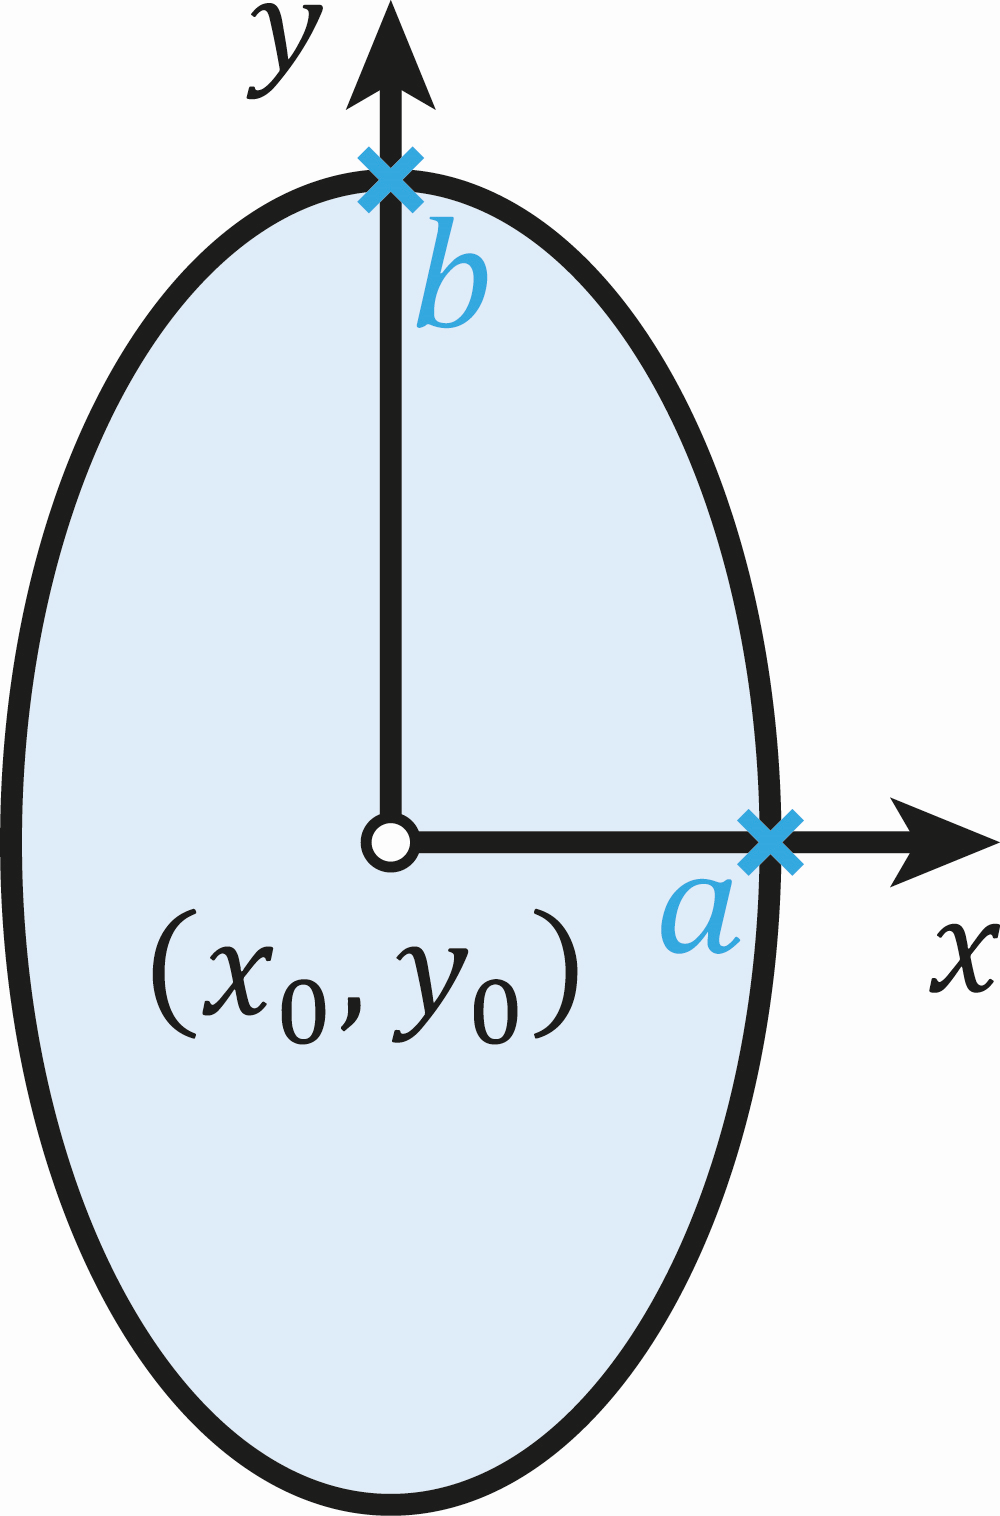
\includegraphics[width=\linewidth, keepaspectratio]{graphics/media/ellipse_skizze.png}
    \tcblower
    \begin{formulabox}
        \textVorFormel{Parametrisiert mit $t \in [0,2\pi]$:}
        $\vec{r}(t) = (x_0 + a\cos(t), y_0 + b\sin(t))$\par
        \tcbline
        \textVorFormel{Implizit:}
        $\frac{(x - x_0)^2}{a^2} + \frac{(y - y_0)^2}{b^2} = 1$
    \end{formulabox}
    \textNachBox{Der Normalenvektor zeigt zum Mittelpunkt der Ellipse.}
\end{splitbox}
\end{defbox}

\begin{defbox}[Hyperbel ($x$-Achsenabschnitt $a$)]
\begin{splitbox}[0.3]
    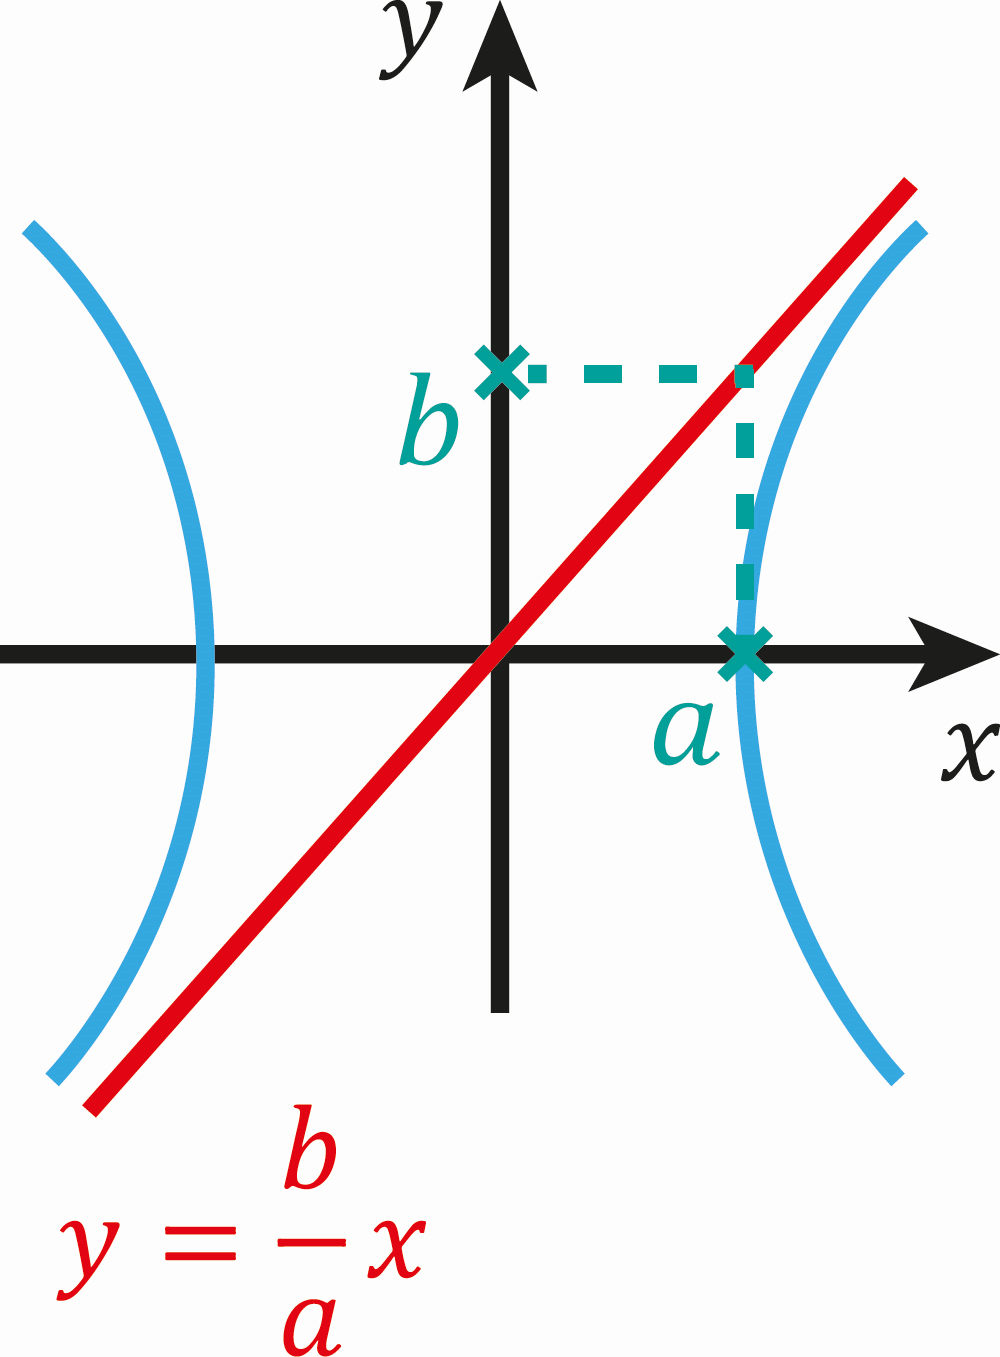
\includegraphics[width=\linewidth, keepaspectratio]{graphics/media/hyperbel_skizze.png}
    \tcblower
    \begin{formulabox}
        \textVorFormel{Parametrisiert mit $t \in [0,2\pi]$:}
        $\vec{r}(t) = (\pm a\cosh(t), y_0 + b\sinh(t))$\par
        \textNachFormel{$y_0$ ist eine Verschiebung in $y$-Richtung.}\par
        \tcbline
        \textVorFormel{Implizit:}
        $\left(\frac{x}{a}\right)^2 - \left(\frac{y}{b}\right)^2 = 1$\par
        \tcbline
        \textVorFormel{Explizit:}
        $f(x) = \pm b\sqrt{\left(\frac{x}{a}\right)^2 - 1}$
    \end{formulabox}
\end{splitbox}
\end{defbox}

\begin{defbox}[Bernoullispirale]
\begin{splitbox}[0.3]
    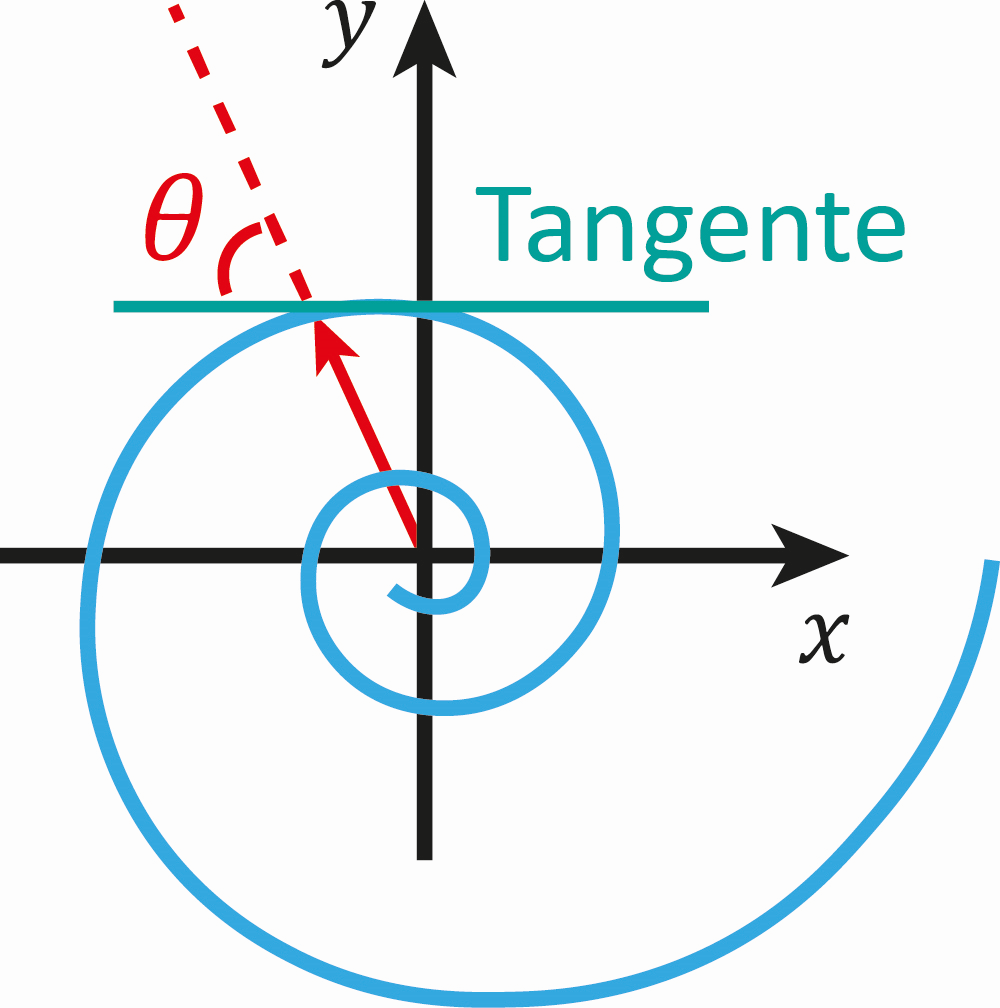
\includegraphics[width=\linewidth, keepaspectratio]{graphics/media/bernoullispirale_skizze.png}
    \tcblower
    \begin{formulabox}
        \textVorFormel{Parametrisiert mit $\varphi \in [0, \infty)$:}
        $\vec{r}(\varphi) = C\left(\cos(\varphi)e^{k\varphi}, \sin(\varphi)e^{k\varphi}\right)$\par
        \tcbline
        $\rho(\varphi) = Ce^{k\varphi}$
    \end{formulabox}
    \textNachBox{Der Winkel $\theta$ zw. Ortsvektor \& Tangente ist konstant. Drehung von $\vec{r}$ um $\pi$: parallele Tangenten.}
\end{splitbox}
\end{defbox}

\begin{defbox}[Zykloide (Kreisradius $a$)]
\begin{splitbox}[0.3]
    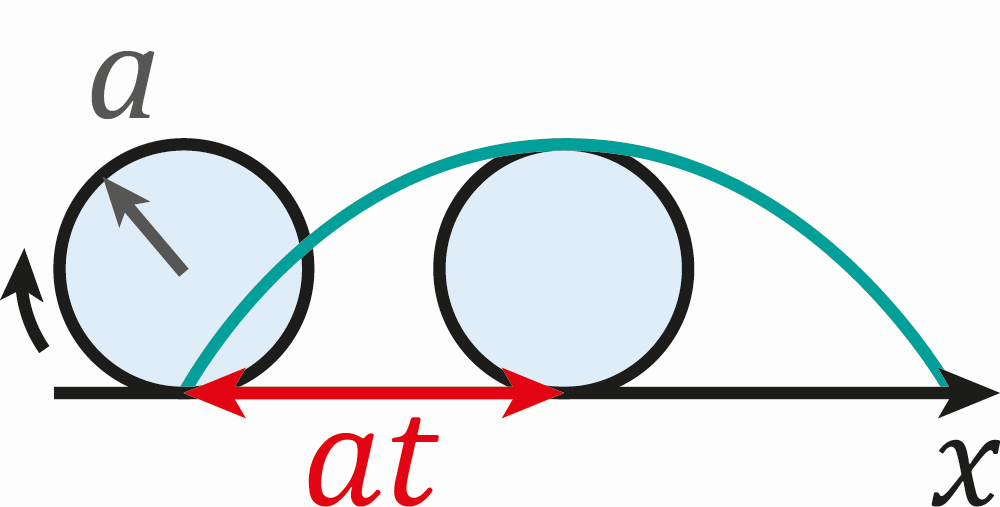
\includegraphics[width=\linewidth, keepaspectratio]{graphics/media/zykloide_skizze.png}
    \tcblower
    \begin{formulabox}
        \textVorFormel{Parametrisiert mit $t \in [0, \infty)$:}
        $\vec{r}(t) = (at - b\sin(t), a - b\cos(t))$
    \end{formulabox}
\end{splitbox}
\textNachBox{\textbf{Verlängerte}: $b > a$, \textbf{Verkürzte}: $b < a$}
\end{defbox}

\begin{defbox}[Astroide (Äusserer Kreisradius $R$, innerer Kreisradius $r$)]
\begin{splitbox}[0.3]
    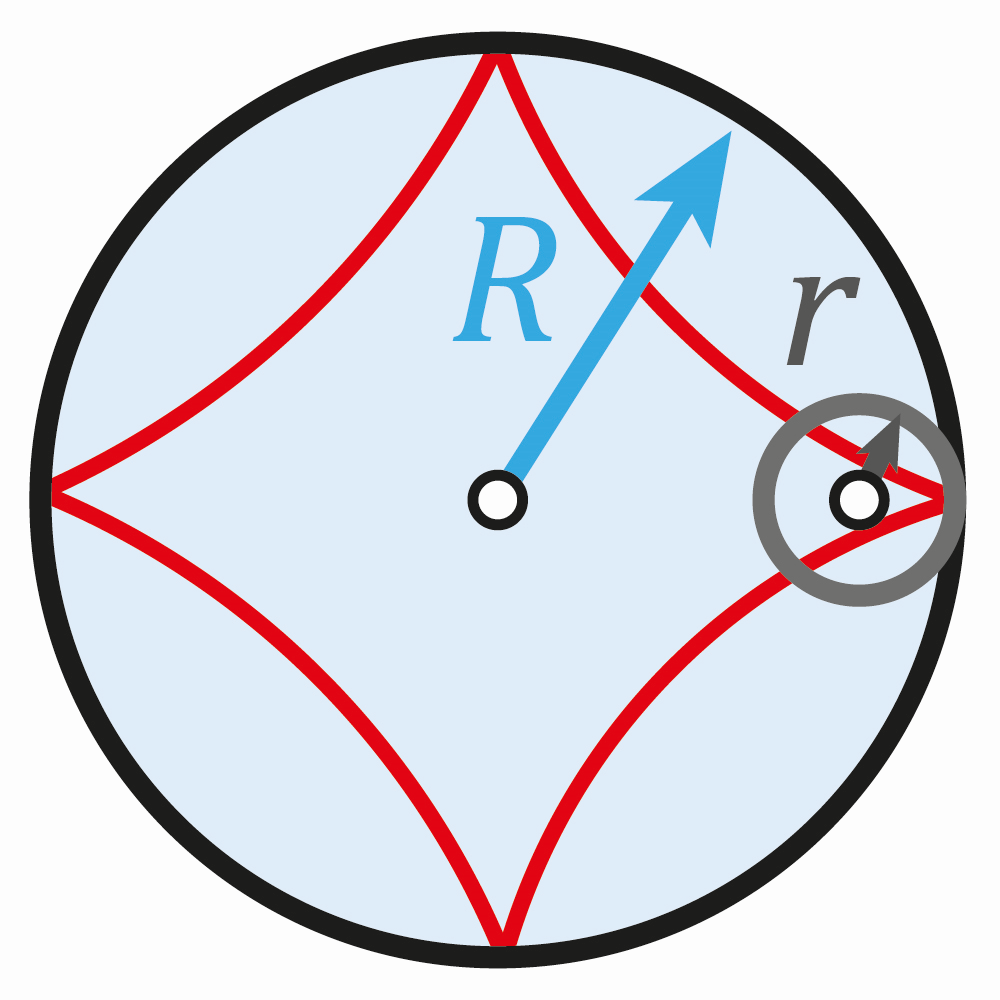
\includegraphics[width=\linewidth, keepaspectratio]{graphics/media/astroide_skizze.png}
    \tcblower
    \begin{formulabox}
        \textVorFormel{Parametrisiert mit $\varphi \in [0,2\pi)$:}
        $\vec{r}(t) = (x_0 + R\cos^3(t), y_0 + R\sin^3(t))$\par
        \tcbline
        \textVorFormel{Explizit:}
        $x^{\frac{2}{3}} + y^{\frac{2}{3}} = R^{\frac{2}{3}}$
    \end{formulabox}
\end{splitbox}
\end{defbox}


\SubsectionBar{Eigenschaften Ebene Kurven\ZSFScriptRef{67}}

\textVorBox{Der \ZSFkeyword{Richtungsvektor} einer parametrisierten Kurve $\vec{r}(t) = (x(t), y(t))$ besitzt folgende Eigenschaften:}

\begin{fulltablebox}{Q{0.8} | Y{1.2}}
    \ZSFrowColor
    Tangentensteigung: & $\displaystyle \frac{\dot{y}(t)}{\dot{x}(t)}$ \\ \hline
    Tangentialvektor: & $\displaystyle \vec{t}(t) = \dot{\vec{r}}(t) = (\dot{x}(t), \dot{y}(t))$ \\ \hline
    \ZSFrowColor
    Tangente an Kurve: & $\displaystyle \vec{t}(t_0) = \vec{r}(t_0) + s\,\vec{t}(t_0)$ \\
\end{fulltablebox}

\textNachBox{Für eine horizontale Tangente gilt $\dot{y}(t) = 0$. Für eine vertikale Tangente gilt $\dot{x}(t) = 0$.}

\textVorBox{\ZSFkeyword{Normale}: Steht orthogonal zur Tangente.}

\begin{fulltablebox}{Q{0.8} | Y{1.2}}
    \ZSFrowColor
    Normalenvektor: & $\displaystyle \vec{n}(t) = (-\dot{y}(t), \dot{x}(t))$ \\ \hline
    nach aussen: & $\displaystyle \vec{n}(t) = (\dot{y}(t), -\dot{x}(t))$ \\ \hline
    \ZSFrowColor
    Normale an Kurve: & $\displaystyle \vec{n}(t_0) = \vec{r}(t_0) + s\,\vec{n}(t_0)$ \\ \hline
    normierter Normalenvektor: & $\displaystyle \hat{n}(t) = \frac{1}{\sqrt{\dot{x}(t)^2 + \dot{y}(t)^2}} \begin{pmatrix} -\dot{y}(t) \\ \dot{x}(t) \end{pmatrix}$ \\
\end{fulltablebox}

\textVorBox{\ZSFkeyword{Bogenlänge}:}
\begin{formulabox}
    $\displaystyle s(t_1, t_2) = \int_{t_1}^{t_2} \sqrt{\dot{x}(t)^2 + \dot{y}(t)^2}\,dt$
\end{formulabox}

\textVorBox{\ZSFkeyword{Krümmung}:}
\begin{formulabox}
    \textbf{Parametrisiert:}\quad $\displaystyle \kappa(t) = \frac{\dot{x}\ddot{y} - \ddot{x}\dot{y}}{(\dot{x}^2 + \dot{y}^2)^{3/2}}$\par
    \formulasep
    \textbf{Explizit:}\quad $\displaystyle \kappa(x) = \frac{f''(x)}{(1 + f'(x)^2)^{3/2}}$\par
    \formulasep
    \textbf{Polarkoordinaten:}\quad $\displaystyle \kappa(\varphi) = \frac{\rho^2 + 2\dot{\rho}^2 - \rho\ddot{\rho}}{(\rho^2 + \dot{\rho}^2)^{3/2}}$\par
\end{formulabox}

\begin{itemize}
    \item Negative Krümmung (konkav) bei einer Rechtskurve, positive Krümmung (konvex) bei einer Linkskurve
    \item Je enger die Kurve, desto grösser die Krümmung
\end{itemize}

\textVorBox{\ZSFkeyword{Krümmungskreis}: Kreis, der die Krümmung einer ebenen Kurve in einem Punkt beschreibt. Sein Radius, der \ZSFkeyword{Krümmungsradius}, ist der Kehrwert der Krümmung:}
\begin{formulabox}
    $\displaystyle R = \frac{1}{|\kappa|}$
\end{formulabox}

\textVorBox{\ZSFkeyword{Krümmungskreismittelpunkte}:}
\begin{formulabox}
    \begin{longformula}
        x_M &= x - \frac{\dot{y}(\dot{x}^2 + \dot{y}^2)}{\dot{x}\ddot{y} - \ddot{x}\dot{y}} \\
        y_M &= y + \frac{\dot{x}(\dot{x}^2 + \dot{y}^2)}{\dot{x}\ddot{y} - \ddot{x}\dot{y}}
    \end{longformula}
\end{formulabox}

\textVorBox{Die \ZSFkeyword{Evolute} einer Kurve ist die Ortskurve aller Krümmungskreismittelpunkte:}
\begin{formulabox}
    \begin{longformula}
        \vec{E}(t) &= \vec{r}(t) + \rho(t) \cdot \vec{m}(t) \\
        &= \left( x - \frac{1}{\kappa(t)} \cdot \frac{\dot{y}(t)}{\sqrt{\dot{x}(t)^2 + \dot{y}(t)^2}}, y + \frac{1}{\kappa(t)} \cdot \frac{\dot{x}(t)}{\sqrt{\dot{x}(t)^2 + \dot{y}(t)^2}} \right)
    \end{longformula}
\end{formulabox}

\begin{splitbox}[0.6]
    \begin{itemize}[leftmargin=*, nosep]
        \item Evolute eines Kreises: Punkt
        \item Evolute einer Astroide: Astroide
        \item Evolute einer Ellipse: Astroide
        \item Evolute einer Parabel: Form einer\par Möwe (Neilsche Parabel)
    \end{itemize}
    \tcblower
    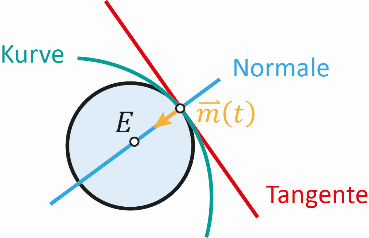
\includegraphics[width=\linewidth, keepaspectratio]{graphics/media/kruemmungskreis_skizze.png}
\end{splitbox}
